\section{Visual Regression Evaluation}

To assess whether agent optimisations introduce perceptible visual changes or functional breakages, we developed a comprehensive, hybrid visual regression pipeline. Given a baseline page $B$ and a candidate page $C$, both are loaded in a headless Chromium browser at a 1280\,px viewport width. The pipeline evaluates regressions across four distinct dimensions:

\textbf{1. Structure-Aware DOM Matching:} Rather than relying solely on pixel-level image diffs, the tool extracts per-element bounding boxes and builds a pruned visual tree. It identifies \emph{section} nodes via a two-pass bottom-up traversal: starting from each leaf, it walks up the DOM seeking the lowest ancestor whose rendered width meets a content-width threshold ($\tau_1 = 0.98$ in the first pass, $\tau_2 = 0.80$ in the second), skipping full-page-width wrappers. A greedy non-overlap filter resolves any candidates with overlapping bounding boxes. Leaf and section nodes from $B$ are matched to their counterparts in $C$ using a heuristic combining text similarity (weight 0.8) and spatial proximity (weight 0.2), reversed for image or empty nodes. A structural regression is flagged when the mean Leaf IoU $< 0.95$, mean Section IoU $< 0.95$, or if any elements are unmatched on either side.

\textbf{2. Textual Similarity:} We extract all visible text tokens from the DOM (excluding scripts and styles) and compute the Jaccard similarity between $B$ and $C$. A text regression is flagged if the similarity score falls below a strict threshold of $0.97$.

\textbf{3. Large Multimodal Model (LMM) Evaluation:} We capture full-page screenshots of both versions and prompt a GPT-4 Vision model acting as a visual QA engineer. The model is instructed to identify explicit visual breakages such as missing content, broken layouts, or severe styling issues, while ignoring minor, intentional layout shifts.

\textbf{4. Console Error Monitoring:} The headless browser actively monitors console logs during page load. A regression is flagged if any new JavaScript errors appear in $C$ that were not present in $B$.

An overall regression flag is raised if \emph{any} of these four checks detect an issue. Using the final trimmed evaluation set of 88 pairs of baseline and patched code generated by 4 agents, the hybrid pipeline flags 42/88 pairs (47.7\%) as regressions and 46/88 pairs (52.3\%) as no regression. Detection rates by agent are: Aider 30.4\% (7/23), Claude Code 47.6\% (10/21), Codex 54.5\% (12/22), and OpenCode 59.1\% (13/22).

To evaluate the tool, we conducted a manual labelling study of the evaluation set. A single annotator ($K=1$) with front-end experience was shown side-by-side renderings of baseline and modified pages and asked whether a perceptible visual change was present, with no access to the underlying HTML\@. Because $K=1$, inter-annotator agreement ($\kappa$) is not applicable.

The individual pipeline signals vary significantly in their sensitivity and alignment with human perception (Table~\ref{tab:vr-agreement}). The structure-aware DOM matching achieves the highest independent agreement with the manual labels (81.8\%). Conversely, the hybrid overall approach behaves aggressively to maximize recall successfully catching 18 of the 20 manual regressions though this sensitivity comes at the cost of a higher false positive rate, dropping overall agreement to 70.5\%. Failures in the pipeline are largely concentrated in cases where a change is spatially confined to a small element, leaving the broader layout intact and IoU scores near the threshold, or on pages with dynamic content where minor positional drift mimics a structural change. Figure~\ref{fig:visual-regressions} illustrates examples of perceptible visual regressions correctly flagged by our tool.

\begin{table}[h]
\centering
\caption{Performance of individual pipeline signals and the overall hybrid tool compared against manual annotations on the 88-pair evaluation set.}
\label{tab:vr-agreement}
\begin{tabular}{lcccccc}
\toprule
\textbf{Signal} & \textbf{Firing Rate} & \textbf{Agreement} & \textbf{TP} & \textbf{FP} & \textbf{TN} & \textbf{FN} \\
\midrule
DOM Structural & 34.1\% (30/88) & 81.8\% & 17 & 13 & 55 & 3 \\
Text Jaccard   & 1.1\% (1/88)   & 78.4\% & 1  & 0  & 68 & 19 \\
GPT-4 Vision   & 15.9\% (14/88) & 79.5\% & 8  & 6  & 62 & 12 \\
Console Errors & 25.0\% (22/88) & 75.0\% & 10 & 12 & 56 & 10 \\
\midrule
\textbf{Hybrid Overall} & \textbf{47.7\% (42/88)} & \textbf{70.5\%} & \textbf{18} & \textbf{24} & \textbf{44} & \textbf{2} \\
\bottomrule
\end{tabular}
\end{table}

\begin{figure}[h]
    \centering
    % Top example
    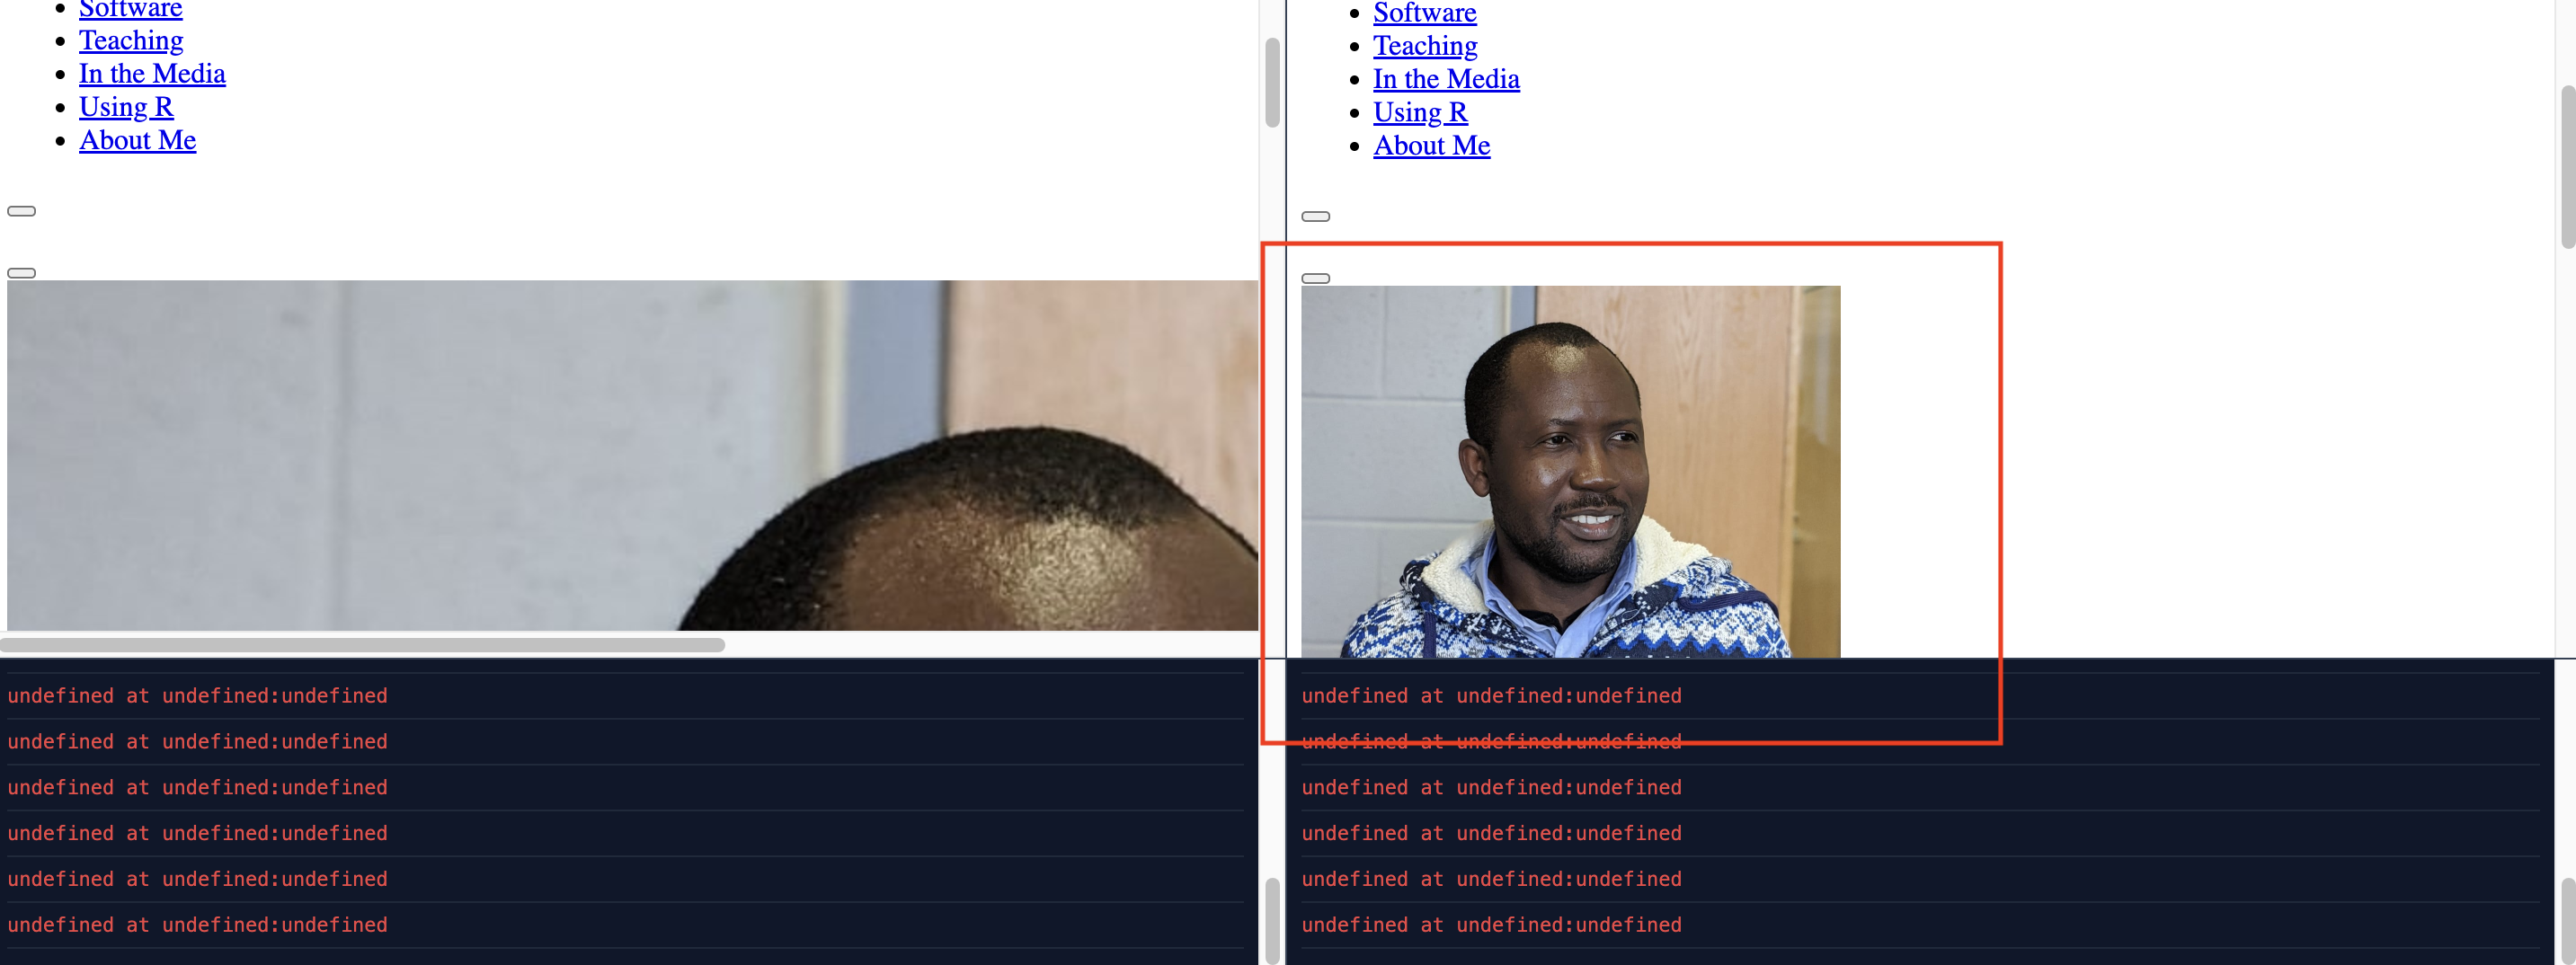
\includegraphics[width=\linewidth]{figures/regression_1.png} \\
    \vspace{0.3cm} % Add some spacing between the two images
    % Bottom example
    
\includegraphics[width=\linewidth]{figures/regression_2.png}
    \caption{Examples of visual regressions detected by the regression tool. Each pair displays the baseline rendering alongside the candidate rendering, highlighting layout shifts, missing content, or styling issues introduced by the optimization agents. The red bounding box depicts the regression area.}
    \label{fig:visual-regressions}
\end{figure}
